\documentclass[11pt,a4paper]{article}
\usepackage[margin=2.2cm]{geometry}
\usepackage{amsmath,amssymb}
\usepackage{graphicx}
\usepackage{booktabs}
\usepackage{tabularx}
\usepackage{caption}
\usepackage{xcolor}
\usepackage{pgfplots}
\pgfplotsset{compat=1.18}
\usepackage[hidelinks]{hyperref}

\newcommand{\figdir}{fig}
\newcommand{\simf}{\operatorname{sim}}

\title{Real-Time Multi-Target Multi-Camera Tracking on NVIDIA DeepStream\\[4pt]
\large Comprehensive Summary Report}
\author{[Student name] \\ Supervisor: [Supervisor name]}
\date{14 November 2026}

\begin{document}
\maketitle

\begin{abstract}
We present a multi-target multi-camera tracking (MTMCT) system that assigns a consistent
\emph{Global ID} to people moving across three IP cameras, covering both overlapping and
non-overlapping fields of view, in real time. Detection, single-camera tracking and
re-identification run in an NVIDIA DeepStream 7.1 pipeline on a GPU; the main contribution is
a GPU-free cross-camera association module that combines appearance, camera topology
(transit-time windows) and ground-plane geometry, solved online with a per-camera Hungarian
assignment. All association parameters are selected with leave-one-session-out (LOSO)
cross-validation on self-recorded data and confirmed on a held-out group of sessions with
harder scenarios. On the selection sessions the final configuration reaches HOTA 79.5,
IDF1 90.4 and 82\% identity-handover accuracy; on the held-out group it reaches HOTA 61.2,
IDF1 67.2 and 57\% handover accuracy, with time-to-Global-ID p95 below 1~s of data time.
\end{abstract}

\tableofcontents

%==============================================================================
\section{Problem and objectives}

Given $M$ cameras, the system must detect every person, track them within each camera, and
link those per-camera tracks (\emph{tracklets}) into identities that persist across cameras.
The deployment targeted by this thesis is a \textbf{mixed} topology:
\begin{itemize}
  \item \textbf{overlapping} pairs, where the same floor area is seen from two angles and
        positions can be compared directly through homographies;
  \item \textbf{non-overlapping} pairs, where people disappear for several seconds and only
        appearance and travel time are available;
  \item \textbf{returns} to the same camera after leaving it.
\end{itemize}
Targets from the proposal: 3--4 streams, $\geq 15$ FPS per stream, and end-to-end latency
below 1~s. Detector and re-identification models are used \emph{pretrained}; the technical
contribution is the association module (\texttt{src/mct/}).

%==============================================================================
\section{System architecture}

The system has three tiers decoupled by Redis Streams (Fig.~\ref{fig:arch}). The only
interface between the GPU pipeline and the association engine is a versioned message schema.
Because the stream can be recorded to a fixture and replayed, every association experiment in
this report runs on a CPU and is bit-for-bit reproducible.

\begin{figure}[h]
  \centering
  \includegraphics[width=\linewidth]{\figdir/01-architecture.pdf}
  \caption{System architecture. The association engine never imports GPU libraries; it reads
  \texttt{mct:frames} and publishes Global IDs to \texttt{mct:global} and SQLite.}
  \label{fig:arch}
\end{figure}

\begin{figure}[h]
  \centering
  \includegraphics[width=\linewidth]{\figdir/02-deepstream-pipeline.pdf}
  \caption{DeepStream pipeline. YOLO11s (COCO, TensorRT FP16) detects people; NvDCF tracks
  them and extracts 512-d OSNet x1.0 embeddings (domain-generalization checkpoint); a pad
  probe rescales boxes, L2-normalizes embeddings and stamps a wall-clock timestamp.}
  \label{fig:pipeline}
\end{figure}

\paragraph{Model choices.} Detector and re-ID weights are not fine-tuned. The pretrained
weights were already trained on the datasets one would fine-tune on (COCO, Market-1501/MSMT17),
and on WildTrack a domain-generalization re-ID checkpoint outperformed a Market-1501-specific
one by $+25\%$ F1 (0.346 vs.\ 0.277). PeopleNet Transformer and YOLO26s were evaluated as
alternative detectors and did not beat YOLO11s (Section~\ref{sec:wildtrack}).

%==============================================================================
\section{Cross-camera association}
\label{sec:method}

Every 500~ms window (data time), each tracklet that has been updated is matched against the set
of active Global tracks (Fig.~\ref{fig:algo}). Notation: tracklet $T$ in camera $c$, Global
track $G$, L2-normalized embeddings $\mathbf f$.

\begin{figure}[p]
  \centering
  \includegraphics[width=\linewidth,height=0.82\textheight,keepaspectratio]{\figdir/03-association-algorithm.pdf}
  \caption{Online association loop, executed every 500~ms of data time.}
  \label{fig:algo}
\end{figure}

\subsection{Ground-plane geometry}
Each camera is calibrated to one shared floor coordinate system with a homography $H_c$
estimated from tape-measured floor points:
\begin{equation}
  \begin{bmatrix} X \\ Y \\ 1 \end{bmatrix} \sim H_c \begin{bmatrix} u \\ v \\ 1 \end{bmatrix},
  \qquad (u,v) = \left(x + \tfrac{w}{2},\; y + h\right).
\end{equation}
When the feet are occluded, the bottom of the box is unreliable. A second homography
$H^{\mathrm{head}}_c$, fitted by least squares on unoccluded boxes, maps the head point to the
ground (\emph{head-plane foot model}):
\begin{equation}
  \mathbf p_{\text{ground}} = H^{\mathrm{head}}_c \begin{bmatrix} x + \tfrac{w}{2} \\ y \\ 1 \end{bmatrix},
  \qquad \hat{\mathbf p}_{\text{image}} = H_c^{-1}\,\mathbf p_{\text{ground}}.
\end{equation}

\subsection{Appearance}
The query embedding of a tracklet is the confidence-weighted mean of its $k=8$
highest-confidence embeddings $\mathcal K$ (not the last frame, which is often blurred or
occluded):
\begin{equation}
  \mathbf q_T = \frac{\sum_{i\in\mathcal K} s_i\,\mathbf f_i}{\bigl\lVert \sum_{i\in\mathcal K} s_i\,\mathbf f_i \bigr\rVert_2}.
\end{equation}
Each Global track keeps a bounded gallery $\mathcal G_G$ ($\leq 32$ embeddings); similarity is
the best match in the gallery:
\begin{equation}
  \simf(T,G) = \max_{\mathbf g \in \mathcal G_G} \mathbf g^{\top}\mathbf q_T .
\end{equation}

\subsection{Ground distance}
Positions are compared \emph{at the same time}, not end-to-start. With $\mathcal S$ the set
of shared timestamps of the two trajectories (tolerance 200~ms):
\begin{equation}
  d_{\text{ground}}(T,G) = \operatorname*{median}_{t \in \mathcal S}
  \bigl\lVert \mathbf p_T(t) - \mathbf p_G(t) \bigr\rVert_2 .
\end{equation}
Without shared timestamps (gap $\Delta t$), a speed gate keeps only physically reachable pairs:
$d \leq d_{\max} + v_{\max}\,\Delta t$ with $d_{\max} = 3$~m and $v_{\max} = 2.5$~m/s.

\subsection{Feasibility constraints}
A cell $(T,G)$ is infeasible ($C=\infty$) if $G$ already owns a tracklet in the same camera
whose time span overlaps $T$ (mutual exclusion), or if the transit time from the last camera
$c'$ falls outside the topology window:
\begin{equation}
  \Delta t \notin \left[t_{\min}^{c' \to c},\; t_{\max}^{c' \to c}\right],
  \qquad \text{e.g.\ } [3.2,\ 19.4]~\text{s for cam01} \leftrightarrow \text{cam03}.
\end{equation}
Windows are measured on dedicated calibration recordings, never on scored sessions.

\paragraph{Soft upper window (session 46).} Diagnosis showed that 12 of 86 first-decision
errors came from people who walked slower than $t_{\max}$ (26--37~s). Late arrivals are
therefore kept, but only with stronger appearance evidence; early arrivals stay infeasible:
\begin{equation}
  \Delta t > t_{\max} \;\Longrightarrow\; \text{feasible} \iff 1 - \simf(T,G) < \tau_{\text{late}} = 0.35 .
\end{equation}

\subsection{Cost and assignment}
\begin{equation}
  C(T,G) = \bigl(1 - \simf(T,G)\bigr) + \lambda\, d_{\text{ground}}(T,G), \qquad \lambda = 0.2 .
\end{equation}
Cells with and without position evidence need opposite thresholds (appearance-only must be
strict; with geometry, tightening appearance only rejects correct pairs), so each cell has
its own budget:
\begin{equation}
  \tau(T,G) =
  \begin{cases}
    0.90 & \text{position evidence (overlap or same-camera stitch)},\\
    0.40 & \text{appearance only}.
  \end{cases}
\end{equation}
The Hungarian algorithm runs \textbf{per camera} on budget-normalized costs; a pair is
accepted when its normalized cost is below one, otherwise a new Global ID is created:
\begin{equation}
  \pi^\star = \arg\min_{\pi} \sum_{T} \frac{C\bigl(T,\pi(T)\bigr)}{\tau\bigl(T,\pi(T)\bigr)},
  \qquad (T,G)\ \text{accepted} \iff \frac{C(T,G)}{\tau(T,G)} < 1 .
\end{equation}
One-to-one matching is only valid within one camera; enforcing it across cameras made a person
seen by $N$ cameras lose $N-1$ tracklets to new IDs (recall 0.06 $\to$ 0.37 when fixed).

\subsection{Deferred revision of the first decision}
Re-ID needs about 1~s of frames to be reliable (rank-1 cross-camera 60\% with the first 5
frames vs.\ 94\% with the whole tracklet), but the latency target forces a decision after
$\approx 0.4$~s. The engine therefore issues a provisional ID immediately at $n_{\min}=5$
frames and revisits it \emph{once} when the tracklet reaches $N$ frames:
\begin{equation}
  G_0 = \pi^\star(T)\big|_{|T| = n_{\min}}, \qquad
  G_1 = \pi^\star\bigl(T \mid \mathbf q_T^{(N)}\bigr), \qquad
  G_1 \neq G_0 \Rightarrow T \text{ moves to } G_1 ,
\end{equation}
with $N = 50$ frames ($\approx 2$~s at 25~fps). Latency is unchanged because the provisional ID
is published at once.

%==============================================================================
\section{Data}

\subsection{WildTrack}
Public dataset, 7 overlapping cameras ($1920\times1080$), annotations on a $12\times36$~m grid.
Used for development and layer-wise error analysis. Nothing is trained on WildTrack.

\subsection{Self-collected lab dataset}
Three Tiandy TC-C131N IP cameras recorded on one laptop (Fig.~\ref{fig:layout}): cam01 and
cam02 overlap over a shared floor area; cam03 covers a corridor 12.4~m away. Every session
therefore contains all three handover types. About 7 consenting participants; video, ground
truth and trajectories never leave the lab machines, and faces are blurred before any image is
published.

\begin{figure}[h]
  \centering
  \includegraphics[width=0.9\linewidth]{\figdir/04-camera-layout.pdf}
  \caption{Lab camera layout and the three handover types.}
  \label{fig:layout}
\end{figure}

\begin{table}[h]
  \centering
  \caption{Scored sessions (annotations at 5~fps; handovers counted per pipeline run).}
  \label{tab:data}
  \resizebox{\linewidth}{!}{%
  \begin{tabular}{llrrrrr}
    \toprule
    Group & Scenario & Sessions & Duration (s) & Overlap & Non-overlap & Return \\
    \midrule
    Selection & s2: non-overlap + return, 2--4 people & 8 & 697 & 35 & 33 & 15 \\
    \midrule
    Held-out & s1: overlap, 1--3 people & 1 & 96 & 8 & 0 & 3 \\
             & s3: crowd, 4--7 people, occlusion & 2 & 166 & 39 & 6 & 11 \\
             & s4: same-colour clothing & 1 & 148 & 10 & 6 & 1 \\
    \midrule
    Total & & 12 & 1107 & 92 & 45 & 30 \\
    \bottomrule
  \end{tabular}}
\end{table}

Each session was processed three times by the real DeepStream pipeline on a rented GPU,
giving 36 metadata fixtures (16{,}596 annotated frames, 18{,}645 ground-truth boxes).

\begin{figure}[h]
  \centering
  \includegraphics[width=\linewidth]{\figdir/05-data-workflow.pdf}
  \caption{Data workflow from recording to scoring.}
\end{figure}

%==============================================================================
\section{Evaluation protocol}

\paragraph{Metrics.} Cross-camera HOTA and IDF1 are computed with TrackEval on a virtual
sequence that concatenates all cameras (AI City Challenge practice), image-box protocol,
IoU~0.5, annotated frames only:
\begin{equation}
  \mathrm{HOTA} = \frac{1}{|\mathcal A|}\sum_{\alpha \in \mathcal A}\sqrt{\mathrm{DetA}_\alpha \cdot \mathrm{AssA}_\alpha},
  \qquad
  \mathrm{IDF1} = \frac{2\,\mathrm{IDTP}}{2\,\mathrm{IDTP} + \mathrm{IDFP} + \mathrm{IDFN}} .
\end{equation}
Because HOTA mixes all cameras, we also report \textbf{handover accuracy} per pair type
$k$, classifying every ground-truth camera transition as correct, split (same person, two IDs)
or wrong (merged with another person):
\begin{equation}
  \mathrm{Acc}_k = \frac{n^{\text{correct}}_k}{n^{\text{correct}}_k + n^{\text{split}}_k + n^{\text{wrong}}_k},
\end{equation}
with a 95\% Wilson interval ($z = 1.96$):
\begin{equation}
  \frac{\hat p + \frac{z^2}{2n} \pm z\sqrt{\frac{\hat p(1-\hat p)}{n} + \frac{z^2}{4n^2}}}{1 + \frac{z^2}{n}} .
\end{equation}

\paragraph{Strict scoring of revisions.} When a decision is revised, the frames already shown
under the provisional ID are scored with that ID, exactly as a dashboard viewer saw them.

\paragraph{Latency.} ``$<1$~s'' means the 95th percentile of both (i) per-frame latency for
people who already have a Global ID and (ii) time from a tracklet's first frame to its first
Global ID, both measured from frame arrival in DeepStream to publication on \texttt{mct:global}.

\paragraph{Leakage-free parameter selection.} The same $\sim$7 people appear in every
session, so nothing is learned from embeddings and nothing is fine-tuned. Only geometry
(foot model) is fitted and only configuration keys are selected from a fixed candidate list
$\Theta$. Selection uses LOSO over the 8 selection sessions $\mathcal S$
(Fig.~\ref{fig:protocol}):
\begin{equation}
  \hat\theta_{-s} = \arg\max_{\theta\in\Theta,\; p_{95}(\theta) < 1\,\mathrm{s}}
  \frac{1}{|\mathcal S| - 1}\sum_{s' \neq s}\mathrm{HOTA}(\theta; s'),
  \qquad
  \mathrm{Score}_{\mathrm{LOSO}} = \frac{1}{|\mathcal S|}\sum_{s\in\mathcal S}\mathrm{HOTA}(\hat\theta_{-s}; s).
\end{equation}
The final configuration is obtained by running the same procedure once on all 8 sessions and
is then scored once on the held-out group, without changes after seeing the result.

\begin{figure}[h]
  \centering
  \includegraphics[width=0.75\linewidth]{\figdir/06-evaluation-protocol.pdf}
  \caption{Evaluation protocol.}
  \label{fig:protocol}
\end{figure}

%==============================================================================
\section{Results}

\subsection{WildTrack: where the error comes from}
\label{sec:wildtrack}
Real pipeline, YOLO11s at 640, $n=3$ runs. Two protocols give numbers that differ by about
$2\times$, so both are reported (Table~\ref{tab:wt}).

\begin{table}[h]
  \centering
  \caption{WildTrack, 400 frames. Ground-plane protocol: in-grid, $T=1$~m.}
  \label{tab:wt}
  \begin{tabular}{lcc}
    \toprule
    Configuration & HOTA (image boxes) & HOTA (ground plane) \\
    \midrule
    YOLO11s 640 + NvDCF + association & $15.79 \pm 0.47$ & $31.1 \pm 0.8$ \\
    PeopleNet Transformer v1.1 & $13.87 \pm 0.33$ & $28.4 \pm 1.1$ \\
    GT boxes + IDs, same engine (oracle) & --- & 63.8 \\
    \bottomrule
  \end{tabular}
\end{table}

Replacing detection and single-camera tracking with ground truth doubles ground-plane HOTA
(31.1 $\to$ 63.8): most of the loss on WildTrack is in the input layers, not in association.
PeopleNet Transformer detects more people, but 84\% of its additional false positives fall
outside the annotated grid; YOLO26s showed no detector-level gain on CPU (recall 0.552 vs.\
0.572). YOLO11s was kept. Numbers are not directly comparable with MV3DT (IDF1 96.5), which
fuses views inside the network and reports on the last 40 frames only.

\subsection{Lab: ablation with LOSO}
Table~\ref{tab:loso} shows the cumulative ablation on the selection group. Each row is the
out-of-sample LOSO score; rows with revision are strictly scored.

\begin{table}[h]
  \centering
  \small
  \caption{LOSO on 8 selection sessions $\times$ 3 runs. Handover counts pooled over folds.}
  \label{tab:loso}
  \resizebox{\linewidth}{!}{%
  \begin{tabular}{lccccccc}
    \toprule
    Configuration & HOTA & AssA & IDF1 & Overlap & Non-ovl. & Return & Total [95\% CI] \\
    \midrule
    Baseline (c0) & 69.9 & --- & --- & 79\% & --- & --- & 70\% \\
    + head-plane foot model & 71.5 & 62.0 & 78.8 & 91\% & 65\% & 53\% & 74\% [68--79] \\
    + embedding quality filter & 71.5 & 62.0 & 78.8 & 91\% & 65\% & 53\% & 74\% [68--79] \\
    + soft transit window & 71.8 & 62.6 & 79.2 & 92\% & 68\% & 53\% & 76\% [70--80] \\
    + deferred revision ($N{=}50$) & \textbf{79.5} & \textbf{75.8} & \textbf{90.4} & \textbf{94\%} & \textbf{80\%} & \textbf{58\%} & \textbf{82\% [77--86]} \\
    \bottomrule
  \end{tabular}}
\end{table}

The embedding quality filter (discarding crops that are occluded or touch the image border)
had no effect and stays disabled: occluded crops already have low detector confidence and
fall outside the top-8, and border crops are often the closest, most informative views.
Revision is the largest single gain, while wrong merges did not increase (18 $\to$ 15) and
time-to-Global-ID was unchanged (p50/p95 439/679~ms).

\subsection{Lab: held-out group}
All rows below use the same 12 fixtures of the held-out group. The last row was run once,
after approval of the configuration. The group had been inspected in earlier sessions, so this
is a repeated check rather than a first-ever blind test.

\begin{table}[h]
  \centering
  \small
  \caption{Held-out group (s1\_1, s3\_1, s3\_2, s4\_1) $\times$ 3 runs.}
  \label{tab:heldout}
  \resizebox{\linewidth}{!}{%
  \begin{tabular}{lccccccc}
    \toprule
    Configuration & HOTA & AssA & IDF1 & Overlap & Non-ovl. & Return & Total [95\% CI] \\
    \midrule
    c0 & 53.4 & 36.6 & 55.7 & 32\% & 44\% & 67\% & 39\% [33--45] \\
    + foot model & 53.0 & 36.0 & 56.0 & 42\% & 53\% & 72\% & 48\% [42--55] \\
    + soft window + revision & \textbf{61.2} & \textbf{47.6} & \textbf{67.2} & \textbf{54\%} & 33\% & \textbf{92\%} & \textbf{57\% [50--63]} \\
    \bottomrule
  \end{tabular}}
\end{table}

\begin{figure}[h]
  \centering
  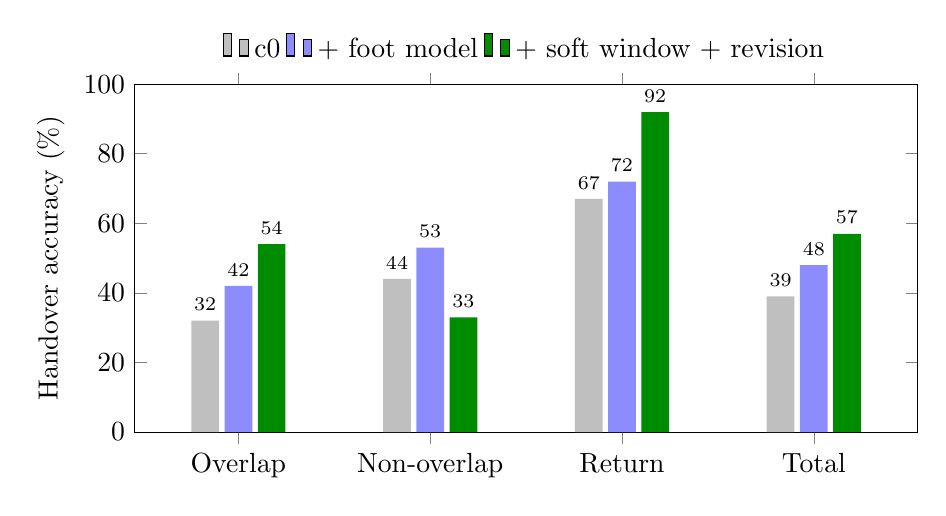
\begin{tikzpicture}
    \begin{axis}[
      ybar, bar width=10pt, width=0.95\linewidth, height=6cm,
      ymin=0, ymax=100, ylabel={Handover accuracy (\%)},
      symbolic x coords={Overlap,Non-overlap,Return,Total},
      xtick=data, enlarge x limits=0.18,
      legend style={at={(0.5,1.03)}, anchor=south, legend columns=3, draw=none},
      nodes near coords, nodes near coords style={font=\scriptsize},
      every axis plot/.append style={draw=none}]
      \addplot[fill=gray!50] coordinates {(Overlap,32) (Non-overlap,44) (Return,67) (Total,39)};
      \addplot[fill=blue!45] coordinates {(Overlap,42) (Non-overlap,53) (Return,72) (Total,48)};
      \addplot[fill=green!55!black] coordinates {(Overlap,54) (Non-overlap,33) (Return,92) (Total,57)};
      \legend{c0, + foot model, + soft window + revision}
    \end{axis}
  \end{tikzpicture}
  \caption{Held-out handover accuracy by pair type.}
  \label{fig:heldout}
\end{figure}

HOTA (+8.2), IDF1 (+11.2), overlap and return handovers improve. \textbf{Non-overlapping
handovers drop from 53\% to 33\%} ($n=36$), opposite to the selection group, and wrong merges
rise slightly (54 $\to$ 57). This could not be reproduced on any selection session, which
points at conditions present only in the held-out scenarios: crowds (s3) and same-colour
clothing (s4), where late matches and revisions rely on appearance that no longer
discriminates. It is reported as a limitation rather than tuned away.

\subsection{Latency and throughput}
Real pipeline on an RTX A4000, 3 streams at 25~fps, YOLO11s 640 + NvDCF + OSNet:
\begin{itemize}
  \item throughput $\approx 176$ FPS per stream, VRAM $\approx 1.2$~GB;
  \item per-frame latency p95 $\approx 205$~ms;
  \item time to Global ID p95 888~ms (12 sessions), or 762~ms excluding the first 3~s of
        pipeline start-up; on the 8 selection sessions with the foot model, p95 1003~ms
        including start-up, the excess coming from people already visible in the first frame.
\end{itemize}

%==============================================================================
\section{Negative results}
Recorded because they explain design decisions:
\begin{itemize}
  \item \textbf{Comparing end point to start point} for overlapping cameras made results worse;
        positions must be compared at shared timestamps.
  \item \textbf{Offline batch association} was \emph{less} accurate than online on WildTrack
        (F1 0.765 vs.\ 0.929): geometry needs trajectories that overlap in time.
  \item \textbf{Evidence time budget} (\texttt{evidence\_max\_gap\_ms}) won on the selection group
        but cost $-7$ HOTA on the held-out group; rejected.
  \item \textbf{Entry zones} reduced return accuracy (53\% $\to$ 40\%); rejected.
  \item \textbf{Embedding quality filter}: no effect (Table~\ref{tab:loso}).
  \item \textbf{Alternative detectors} (PeopleNet Transformer, YOLO26s): not better.
\end{itemize}

%==============================================================================
\section{Limitations and future work}
\begin{itemize}
  \item Selection sessions are sparse (2--4 people); held-out scenarios are much harder, and
        the non-overlap drop there is not yet explained.
  \item The held-out group has been inspected several times; further improvements need newly
        recorded test sessions.
  \item About 7 participants appear in all sessions, which rules out fine-tuning on lab data.
  \item The cam02$\leftrightarrow$cam03 transit window is a placeholder (not measured).
  \item Homography error reaches $\approx 0.7$~m far from the cameras, comparable to the distance
        between two people walking side by side.
\end{itemize}
Next steps: diagnose returns to the same camera (58\% on the selection group, the largest
remaining error), record new test sessions, and measure wall-clock latency on the GPU with
the final configuration.

\end{document}
